\chapter{Exercises with answers}

\begin{Exercise} [
  title={Coding sequence},
  difficulty={1},
  label={excs},
  origin={G. Valle}
 ]
 
 \begin{figure}[H]
  \centering
  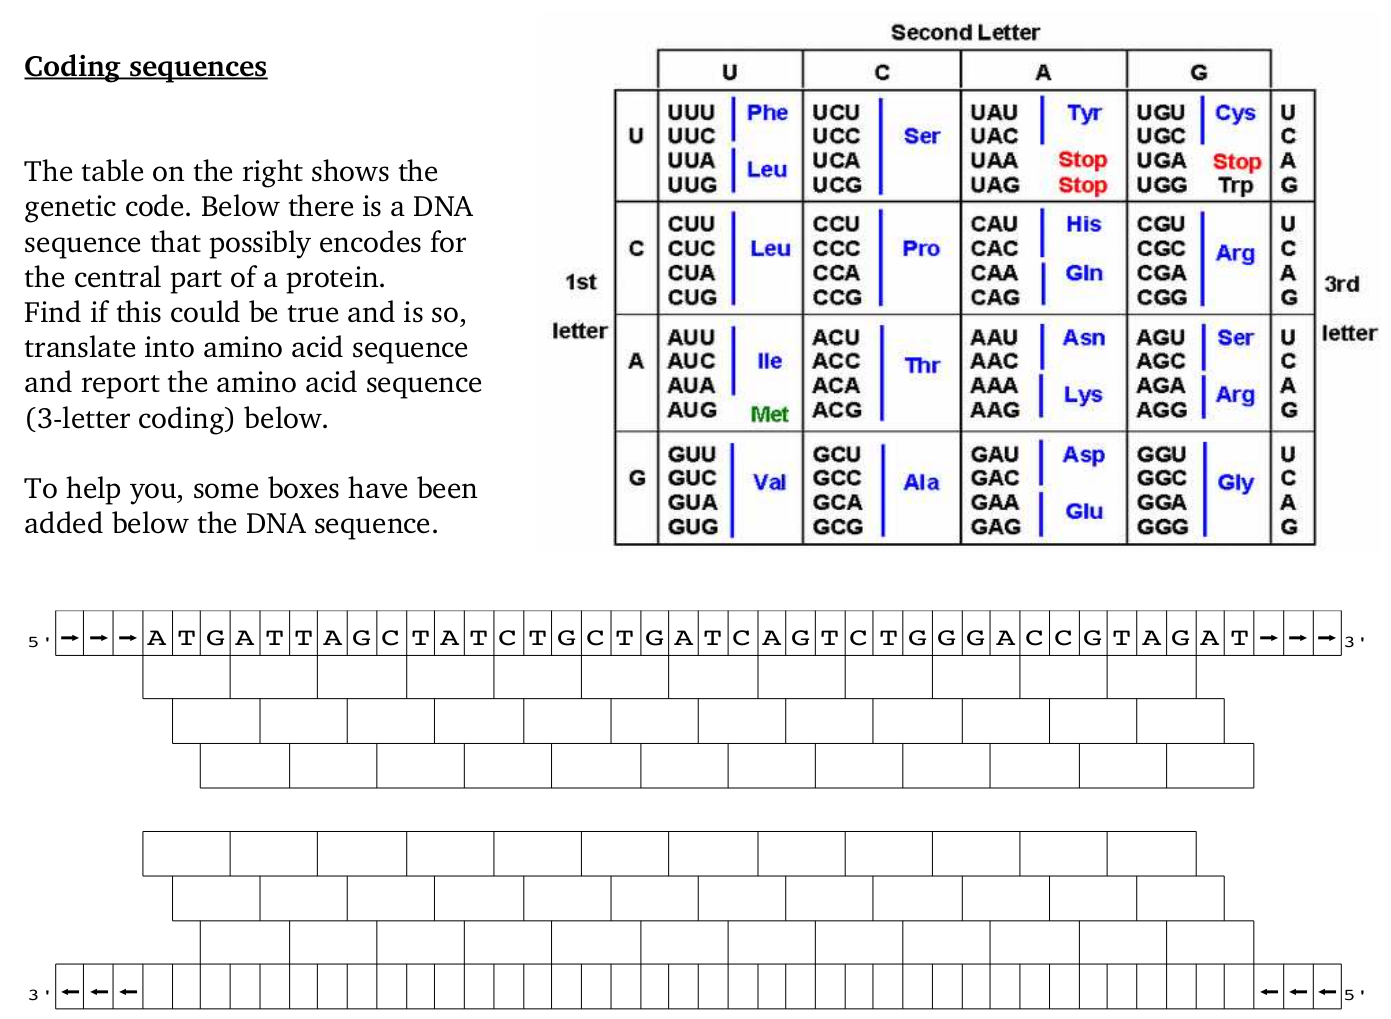
\includegraphics[scale=0.3]{Find_coding_sequence}
 \end{figure}

\end{Exercise}

\newpage

\begin{Answer} [
  ref={excs},
  number={1}
 ]
 
 \begin{figure}[H]
  \centering
  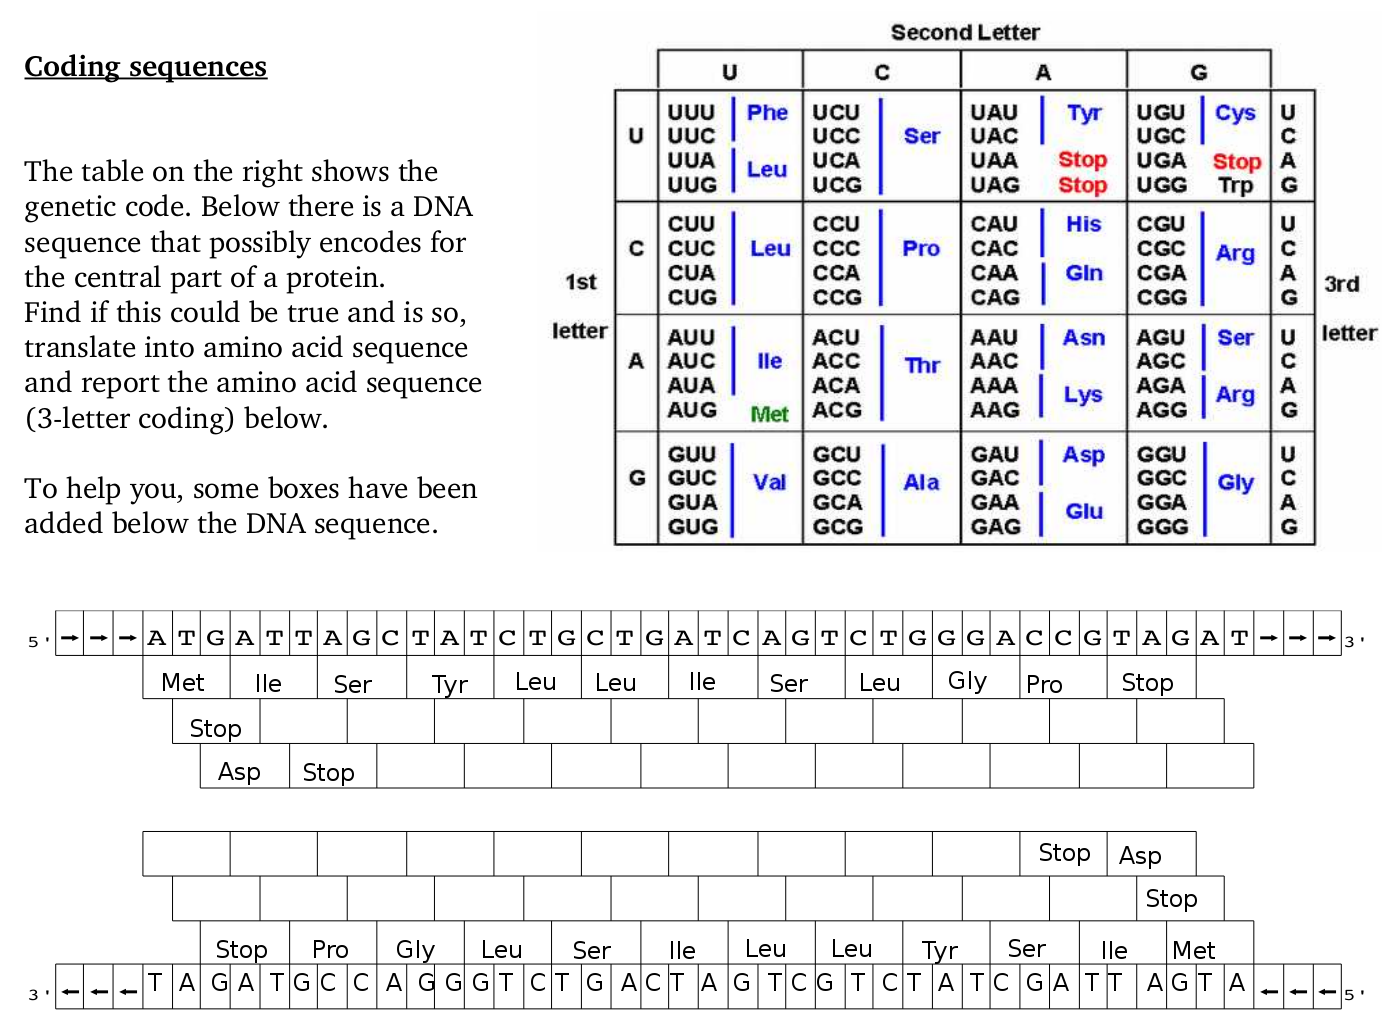
\includegraphics[scale=0.3]{Find_coding_sequence_sol}
 \end{figure}

\end{Answer}



\begin{Exercise} [
  title={Chromosomes},
  difficulty={1},
  label={ex1},
  origin={G. Valle}
 ]

  In adult human cells there are 46 chromosomes. De novo mutations are generally
very rare and we are not considering them in the following reasoning.
Answer \textbf{True} or \textbf{False}:

  \Question 23 chromosome are inherited from the mother and 23 from the father
  \Question Each chromosome of a child must have an identical copy in one of the
2 parents
  \subQuestion Explain why
\end{Exercise}

\begin{Answer} [
   ref={ex1},
   number={1}
 ]

  \Question True
  \Question False
  \subQuestion The second statement is wrong because of the crossing over

\end{Answer}


\begin{Exercise} [
  title={Genomes and genes},
  difficulty={1},
  label={ex2},
  origin={G. Valle}
 ]

  Approximately, how big is the genome and how many genes are there...

  \Question In a bacterium like \textbf{E. Coli}
  \Question In a simple eukaryote like \textbf{yeast}
  \Question In humans

\end{Exercise}

\begin{Answer} [
  ref={ex2},
  number={2}
 ]

  \Question Genome size: 100 Mbp. Number of genes: 19000 (27\% encoding)
  \Question Genome size: 13 Mbp. Number of genes: 6000 (70\% encoding)
  \Question Genome size: 3000 Mbp. Number of genes: 23000/25000 (1.5\% encoding)

\end{Answer}

\begin{Exercise} [
  title={Enzyme},
  difficulty={1},
  label={ex3},
  origin={G. Valle}
 ]

  Answer the questions.

  \Question How is called the enzyme that duplicate the DNA?
  \Question How is called the enzyme that transcribes DNS into RNA?
  \Question How is it called the biological structure where proteins are
synthesized?
\end{Exercise}

\begin{Answer} [
  ref={ex3},
  number={3}
 ]

  \Question DNA Polymerase
  \Question RNA Polymerase
  \Question Ribosome
\end{Answer}
